%%%%%%%%%%%%%%%%%%%%%%%%%%%%%%%%%%%%%%%%%%%%%%%%%%%%%%%%%%%%%%%%%%
%%%%%%%% CPSC 66 FALL 2021  REPORT %%%%%%%%%%%%%%%%%%%%%%%%
%%%%%%%% This template is modified from ICML 2014 %%%%%%%%%%%%%%%%
%%%%%%%%%%%%%%%%%%%%%%%%%%%%%%%%%%%%%%%%%%%%%%%%%%%%%%%%%%%%%%%%%%

\documentclass{article}

%include any external packages here.  This is similar to loading a
%library in python or C++

% use Times
\usepackage{times}
% For figures
\usepackage{graphicx}
  \graphicspath{ {./images/} }
\usepackage{subfigure}

% For citations
\usepackage{natbib}

% For algorithms and pseudocode
\usepackage{algorithm}
\usepackage{algorithmic}

%Adds hyperlinks to your citations automatically
\usepackage{hyperref}

% Packages hyperref and algorithmic misbehave sometimes.  We can fix
% this with the following command.
\newcommand{\theHalgorithm}{\arabic{algorithm}}

\usepackage[accepted]{icml2014}


% If your title is long (below), use this command to also provide
% short version.  This will go on the top of every page
\icmltitlerunning{Final Report}

\begin{document}

\twocolumn[ %use two column if you need a text to span across the whole page
\icmltitle{ CPSC 66 Final Report: \\ % \\ force a new line
Classifying Texts by Time Period }

\icmlauthor{Zachary Kelly}{zkelly1@swarthmore.edu}
\icmlauthor{Sasha Casada}{scasada1@swarthmore.edu}
\icmlauthor{Nathan Le}{nle1@swarthmore.edu}

\vskip 0.3in
]


% Need:
%%  the problem you are addressing *  
%% why the reader should care about this problem * 
%% the algorithms/methods for approaching this problem * 
%% and the main results and/or contributions of your work

\begin{abstract}
  This project aims to classify historical texts by their  
  period of writing, useful in digital humanity studies, such as 
  history, anthropology, political science, and other fields, wherein
  dates of important documents remain unidentified. Traditional methods of classifying texts by time 
  period require human experts with extensive knowledge of 
  history and literature, which can be time-consuming and expensive.
  In our project, we investigated the effectiveness of 
  the Naive Bayes, Random Forest, and ADABoost models as accurate, precise,
  and efficient solutions to these problems. Using $n_{EXAMPLES}\approx 2000$ examples
  spanning $n_{CLASSES}=z$ classes, namely, $>1700s$,$1700-1799$,$1800-1899$, $1900-2000$, $>2000$. 
  We found all models to have some predictive capability, with $Random Forests$
  performing the best, $AdaBoost$ performing below, but with potential for better performance, and $Naive Bayes$
  performing the worst among the three. 

\end{abstract}

\section{Introduction}
\label{introduction}

% What and Why
This paper explores the effectiveness of three supervised ML models at classifying 
the time period of English written works. Given the broad potential application for this, 
it could prove to useful in a number of fields. In developing our research, we primarily 
considered the field of Historical Dating; wherein historians sometimes find themselves 
unable to date an important document, or determine the author of a particular work from a 
few probable candidates due to the unavailability of a definite date of completion, etc. 
Accordingly we carefully designed our classification system with both of these problems in mind. 

In order to accomplish this goal: We collected approximately $2000$ unique 
  English texts dating from \emph{pre-18th} century to \emph{21st} century in the 
  public domain from Project Gutenberg. We extracted features from this raw data
  relating to word-frequency, namely Bag-of-Words (BoW) and Short For-Term-Frequency 
  Inverse Document Frequency (TF-IDF).

The three models we chose for this analysis are
  Naive Bayes, Random Forest, and ADABoost. There has been extensive research 
  into the application of Deep Learning to perform a variety of text-based 
  tasks, but we wanted to explore the value use of these algorithms for this task
  due to their simplicity to implement, run, and test compared to Deep
  Learning Methods, especially with a relatively small and limited dataset. 


%Details of each algorithm and method you applied to the problem
% at a algorithmic level
% That is, tell us what a support vector machine is before 
% telling us how you applied it to your data

% Your methods should include figures and/or pseudocode to help illustrate the approach
% Your methods should include figures and/or pseudocode to help illustrate the approach

\section{Methods}
\label{methods}

\subsection{Naive Bayes}

The Naive Bayes model is a supervised model inherently based on Bayes' Theorem, that is, the 
probability of some event based on past information. It makes two fundamental 
assumptions, that is: 
\begin{enumerate}
  \item Each feature is independent of the others.
  \item Each feature makes an equal contribution. 
\end{enumerate}

Because Naive Bayes makes the assumption that all features are independent makes the algorithm
  very fast compared to other algorithms for classification. For this reason in particular, it 
  is most commonly applied to the task of classification of high-dimensional data (such as text 
  classification). However, all features being independent of each other is not something that
  is often true in real life, thus the algorithm is often considered to be less accurate than
  other similar algorithms.


\subsection{Random Forest}

The Random Forest model is a supervised, ensemble model made up of a grouping of $k$ decision trees that 
are created using randomly selected subsections of the training data. A given 
novel example $a$ is fed to the decision trees, their classifications are made, and
the plurality decision is taken from their results.


There are a few properties of the Random Forest classifier that were desirable for
  our task: 
  \begin{enumerate}
    \item Can handle high-dimensional data well. 
    \item Reduces overfitting; attributed to bagging and random feature selection. 
    \item It is rather robust against noise. Because text data can be noisy and 
      contain irrelevant features, we would like an algorithm that can identify 
      that most relevant features in the classification task.
  \end{enumerate}

\subsection{AdaBoost}

The AdaBoost model (short for: Adaptive Boosting) is a supervised, ensemble model made up of $k$ decision stumps, that
is, trees of depth $1$. It attempts to build a stronger, more effective 
classifier from the $k$ weaker classifiers. It does this by a cycle wherein it 
builds a model from the training data, then builds another model that improves 
upon the errors of the first one. This loop continues until all of the examples 
in the training set are predicted correctly or the loop reaches a max number 
of models. 

Similar to above, there are also features specific to AdaBoost that we identified to be
  helpful in our task, key among them being its handling of class-imbalance. 
  Present in our data-set are several imbalanced 
  classes with labels that sometimes appear significantly more than others. Because
  of the minority class weight-assignment and use of weak classifiers, it can help 
  us with those instances.

\section{Experiments and Results}

\subsection{Data Collection}

Requiring a large amount of English texts spanning a large period of time, 
  we decided to use texts from the online Project Gutenberg Digital Archive. 
  This site serves as an archive of digitized works currently in the public
  domain from a variety of fields, genres, and time periods. We utilized the
  open source (GPL-3.0) \href{https://github.com/pgcorpus/gutenberg}{Standardized 
  Project Gutenberg Corpus (SPGC)} on GitHub in order to automatically scrape the 
  text content and metadata associated with each UTF-8 work available on the site 
  into a CSV. An additional script downloaded all of the works, provided word 
  counts for each work, as well as tokenized versions.

\subsection{Tokenization}

For each work, we made use of the tokenized texts for our data 
  processing. Tokenization is a crucial step for tasks involving Natural Language 
  Processing (NLP). It can be best described as the process for systematically breaking 
  down a text into units (often called words, or subwords) which are used as inputs for 
  various computational tasks, and in our case, feature extraction. To illustrate the 
  concept, consider a text file which contains the following text:

    \hspace{0.5cm} \hangindent=0.65cm \textit{``Lorem ipsum dolor sit amet, consectetur adipiscing}
    \hspace{0.5cm} \textit{elit, sed do eiusmod tempor incididunt ut labore et dolore magna aliqua\dots"}

  Tokenizing the above text and and exporting this text to a file would get you the following:
    \lstset{style=mystyle}
    \hspace{0.5cm} \begin{lstlisting}[language=Python, caption=Tokenization Example]
  lorem 
  ipsum 
  dolor 
  sit 
  amet
  consectetur
  ...
      \end{lstlisting}

Now with individual words on each newline, as well as getting rid of any unnecessary whitespace, 
  symbols, capitalization, etc. we become more easily able to process the the content of the text.

\subsection{Data Processing}

Once we collected and labeled sufficient data for our project, we took a number of steps to process 
  the texts. Firstly, we removed all non-English texts. As our 
  primary goal was to predict the time period of English text,
  we removed all works translated to English from another language more than a decade past their 
  original publication date so as to prevent these texts from 
  interfering with our classifiers' learning processes and/or affecting their
  validation results. 

Next, we fine tuned our data to exclude duplicate texts, anthropologies 
  and compilations of texts published over a period of time. The former to ensure 
  these duplicates did not affect the learning of our classifiers
  or artificially inflate our dataset, and the latter was because of the nature of these texts, 
  their contents would not necessarily accurately reflect their publication year.

When we arrived at an English-only, duplicate-free corpus, we then manually labeled all of our examples by 
using Google Scholar to find the ground-truth publication dates 
of the texts. 
We believed this necessary because, although Project Gutenberg kept detailed information on 
the publication dates of all entries, these sometimes did not align with the true publication date 
of the text. For instance, although \textit{The Magna Carta} has been republished several times,
thus there were several entries for it in the original dataset, none of which
with publication dates that were its correct publication date. 

Then, we assembled approximately $100$ texts into a single document and tokenized it. This was in order 
to produce a feature vector of standardized order by representing each bucket of the vector as 
a word ordered by its frequency. This would allow us to then feed other texts into 
the same feature generation algorithms and compare them with each other, as the features of 
a given text would be in the same order as the others. The implementation for this can be seen at 
\verb|code/generate_wordFrequency.py| and is exported to \verb|code/data|.

% MAKE SURE TO EXPLAIN WELL IN PRESENTATION

\subsection{Feature Generation}

We implemented two word vectorization algorithms that would assign a numeric 
  feature value for a given word $w$ in the vector. The vector is constructed such that 
  words occurring with a higher frequency in the subsample text occur earlier in the vector.

\subsubsection{Bag of Words (BoW)}

Bag-of-Words (Bow) is a numerical classification model where the frequency of occurrence of each word is 
  used as a feature for training a classifier. In this case, each feature represents the total 
  number of occurrences of a particular word in a text, in this case the subsample text.

  To illustrate Bag of Words (BoW), consider the figure below which models the following two sentences:
  
  Ex. 1 \textit{``The dog sat, the cat sat too.''}
  
  Ex. 2 \textit{``The dog and the cat and the other cat all sat.''}

  \vspace{-0.15cm}
  \begin{center}
    \begin{tabular}{ | m{1.2cm} | m{1.2cm}| m{1.2cm} | m{1.2cm} | m{1.2cm} | } 
      \hline
      Text \# & $f_0$ `the' & $f_1$ `dog' & $f_2$ `cat' & $f_3$ `sat' \\ 
      \hline
      Ex. 1 & 2 & 1 & 1 & 1 \\ 
      \hline
      Ex. 2 & 3 & 1 & 2 & 1 \\
      \hline
    \end{tabular}
    \end{center}

\subsubsection{Term-Frequency Inverse Document Frequency (TF-IDF)}

Is a numerical statistic that is intended to reflect how important a word is to a document 
  in a collection or corpus. TF-IDF value increases proportionally to the number of times a 
  word appears in the document and is offset by the number of documents in the corpus that 
  contain the word.

This can be expressed mathematically as:
\vspace{-0.1cm}
\begin{large}
  $$W_{i,j}=tf_{i,j}\times \log{\frac{(N)}{df_i}}$$
\end{large}

\subsection{Data Generation, Train, and Test Pipeline}
We used 1850 example texts, with a total of 20,000 features. We vectorized these using TF-IDF, 
which came out to be the more effective (in terms of accuracy), vectorization algorithm as 
compared to Bag of Words. For labels, we went and used century-long periods for our slicing, 
and we removed stopwords from our vectorization output. Stopwords are usually very 
common words that appear frequently in a language and do not add much meaning to the text, 
such as "the", "a", "an", "and", etc. 

Once we generated our data, we ran our dataset through our three algorithms, as described above, 
with validation.


\subsection{Validation}

<<<<<<< HEAD
\subsubsection{Naive Bayes Classifer}
  Hyperparameter tuning was performed on the $alpha$ parameter across the range $(0, 1]$ This parameter
  space was explored with Randomized Search with 10 sampling iterations and 3 fold cross validation. 

\begin{figure}[h]
  \centering
  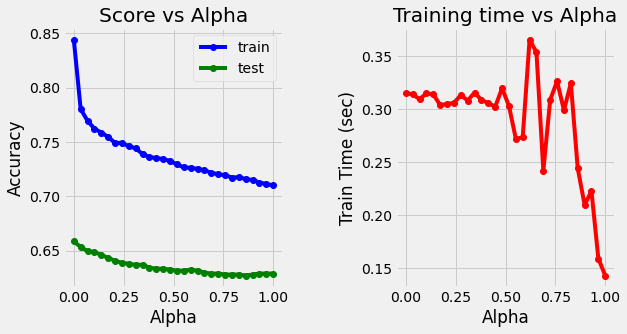
\includegraphics[width=0.5\textwidth]{naivebayes_validation_curve.png}
  \caption{Validation curve of $alpha$ for Naive Bayes Classifier}
  \end{figure}

\begin{table}[ht]
\centering
\caption{tuned parameters for naive bayes}
\begin{tabular}{l|c}
\toprule
parameter & value \\
\midrule
alpha & 0.011633196056020756 \\
\bottomrule
\end{tabular}
\end{table}

\subsubsection{Random Forest Classifer}

Hyperparameter tuning was performed on the following parameters:
\begin{itemize}
\item $n\_estimators$: the number of trees in the forest, with a range from 200 to $\frac{Num Features}{3}$.
\item $max\_features$: the number of features to consider when looking for the best split, with options 'auto' and 'sqrt'.
\item $max\_depth$: the maximum number of levels in the tree, ranging from 10 to 110.
\item $min\_samples\_split$: the minimum number of samples required to split a node, with a range of values $[2, 10]$.
\item $min\_samples\_leaf$: the minimum number of samples required at each leaf node, with a range of values $[1, 4]$.
\item $bootstrap$: the method of selecting samples for training each tree, with options of either True or False.
\end{itemize}

This hyperparameter space was explored with Random Search with 10 sampling iterations and 3 fold cross validation.

\begin{figure}[h]
  \centering
  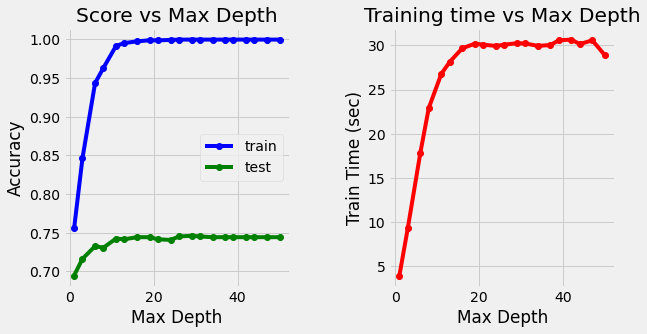
\includegraphics[width=0.5\textwidth]{rf_max_depth.png}
  \caption{Validation curve of $max\_depth$ for Random Forest Classifier}
  \end{figure}

\begin{figure}[h]
  \centering
  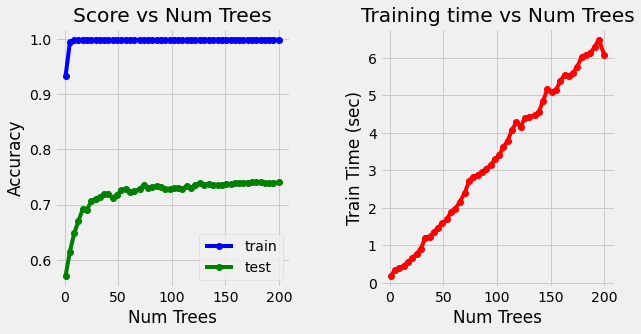
\includegraphics[width=0.5\textwidth]{rf_num_trees.png}
  \caption{Validation curve of $n\_estimators$ for Random Forest Classifier}
  \end{figure}

\begin{table}[ht]
\centering
\caption{tuned parameters for Random Forest Classifier}
\begin{tabular}{l|c}
\toprule
parameter & value \\
\midrule
$n\_estimators$ & 918 \\
$min\_samples\_split$ & 10 \\
$min\_samples\_leaf$ & 1 \\
$max\_features$ & sqrt \\
$max\_depth$ & 60 \\
$bootstrap$ & False \\
\bottomrule
\end{tabular}
\end{table}

\subsubsection{AdaBoost Classifer}

Hyperparameter tuning was performed on the following parameters for the AdaBoost classifier:
\begin{itemize}
\item $n_estimators$: the number of weak learners to train iteratively, with a range from 50 to 500.
\item $learning_rate$: the learning rate, which determines the contribution of each weak learner, ranging from 0.001 to 1.0.
\item $base_estimator$: the type of base estimator used as a weak learner, in this case, a decision tree classifier with varying maximum depths from 1 to 15.
\end{itemize}

This parameter space was explored with Random Search with 10 sampling iterations and 3 fold cross validation.

\begin{figure}[h]
  \centering
  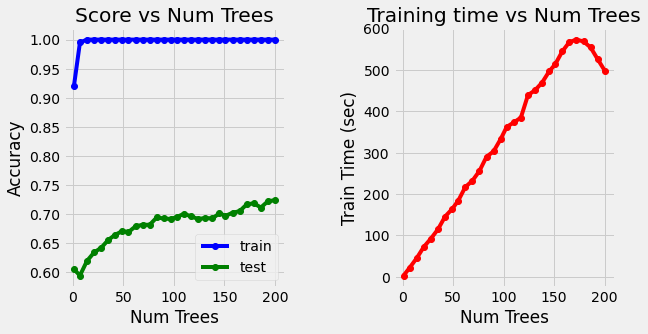
\includegraphics[width=0.5\textwidth]{adaboost_num_trees.png}
  \caption{Validation curve of $n\_estimators$ for AdaBoost Classifier}
  \end{figure}

\begin{table}[ht]
\centering
\caption{Tuned Parameters for AdaBoost Classifier}
\begin{tabular}{l|c}
\toprule
Parameter & Value \\
\midrule
$n\_estimators$ & 250 \\
$learning\_rate$ & 0.9388367346938776 \\
$base\_estimator$ & $max\_depth=7$ \\
\bottomrule
\end{tabular}
\end{table}

\subsection{Results}

Accuracy was used as the primary performance metric for our three models. After parameter
tuning, the performance changes are as follows:

\begin{table}[ht]
\centering
\caption{Model Performance}
\begin{tabular}{l|c|c|c}
\toprule
Model & Base & Tuned & Performance Delta \\
\midrule
AdaBoost & 0.5189 & 0.7270 & 0.2081 \\
Naive Bayes & 0.6527 & 0.7054 & 0.0527 \\
Random Forest & 0.7568 & 0.7773 & 0.0205 \\
\bottomrule
\end{tabular}
\end{table}

The Naive Bayes and Random Forest models experienced rapidly diminishing returns on increasing
model complexity for higher accuracy. It is possible that AdaBoost can be fitted with a greater
number of estimators for higher accuracy, if not for the high computational runtime.

The confusion matrices for the models are as follows:

\begin{figure}[h]
  \centering
  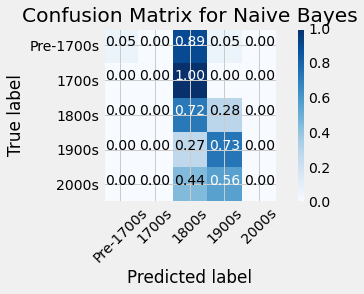
\includegraphics[width=0.5\textwidth]{cm_nb.png}
  \caption{Confusion Matrix for Naive Bayes Classifier}
  \end{figure}

\begin{figure}[h]
  \centering
  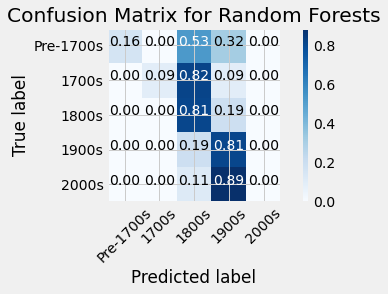
\includegraphics[width=0.5\textwidth]{cm_rf.png}
  \caption{Confusion Matrix for Random Forest Classifier}
  \end{figure}

\begin{figure}[h]
  \centering
  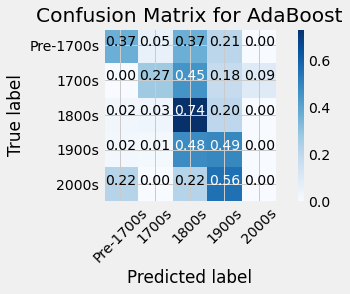
\includegraphics[width=0.5\textwidth]{cm_adaboost.png}
  \caption{Confusion Matrix for AdaBoost Classifier}
  \end{figure}

All three models show that their predictions heavily bias towards either the 1800s or the 1900s. This not
surprising given the high class imbalance of our dataset.

The confusion matrices for the Naive Bayes and Random Forest classifiers imply these models are splitting
their predictions predominantly between texts $<1700s-1899$ and $1900->2000s$ with decent accuracy. This
implies that although these models can capture differences between these two time periods, the models struggle
at making higher resolution classifications.

The AdaBoost confusion matrix shows that, though its predictions bias towards $1800s$ or $1900s$, it is
able to somewhat accurately classify texts outside of the $1800$ and $1900$ range. Notably, it does a
decent job at classifying texts $<1700$ and $1700-1799$. This implies that, despite the class imbalance,
the AdaBoost classifier is able to model some time specific patterns of older texts.

We can inspect the patterns these trees are modeling by examining the feature importance
of the Random Forest and AdaBoost classifiers. The following graphs represent the Gini Impurity / Mean Decrease in Impurity
for the features of the classifiers.

\begin{figure}[h]
  \centering
  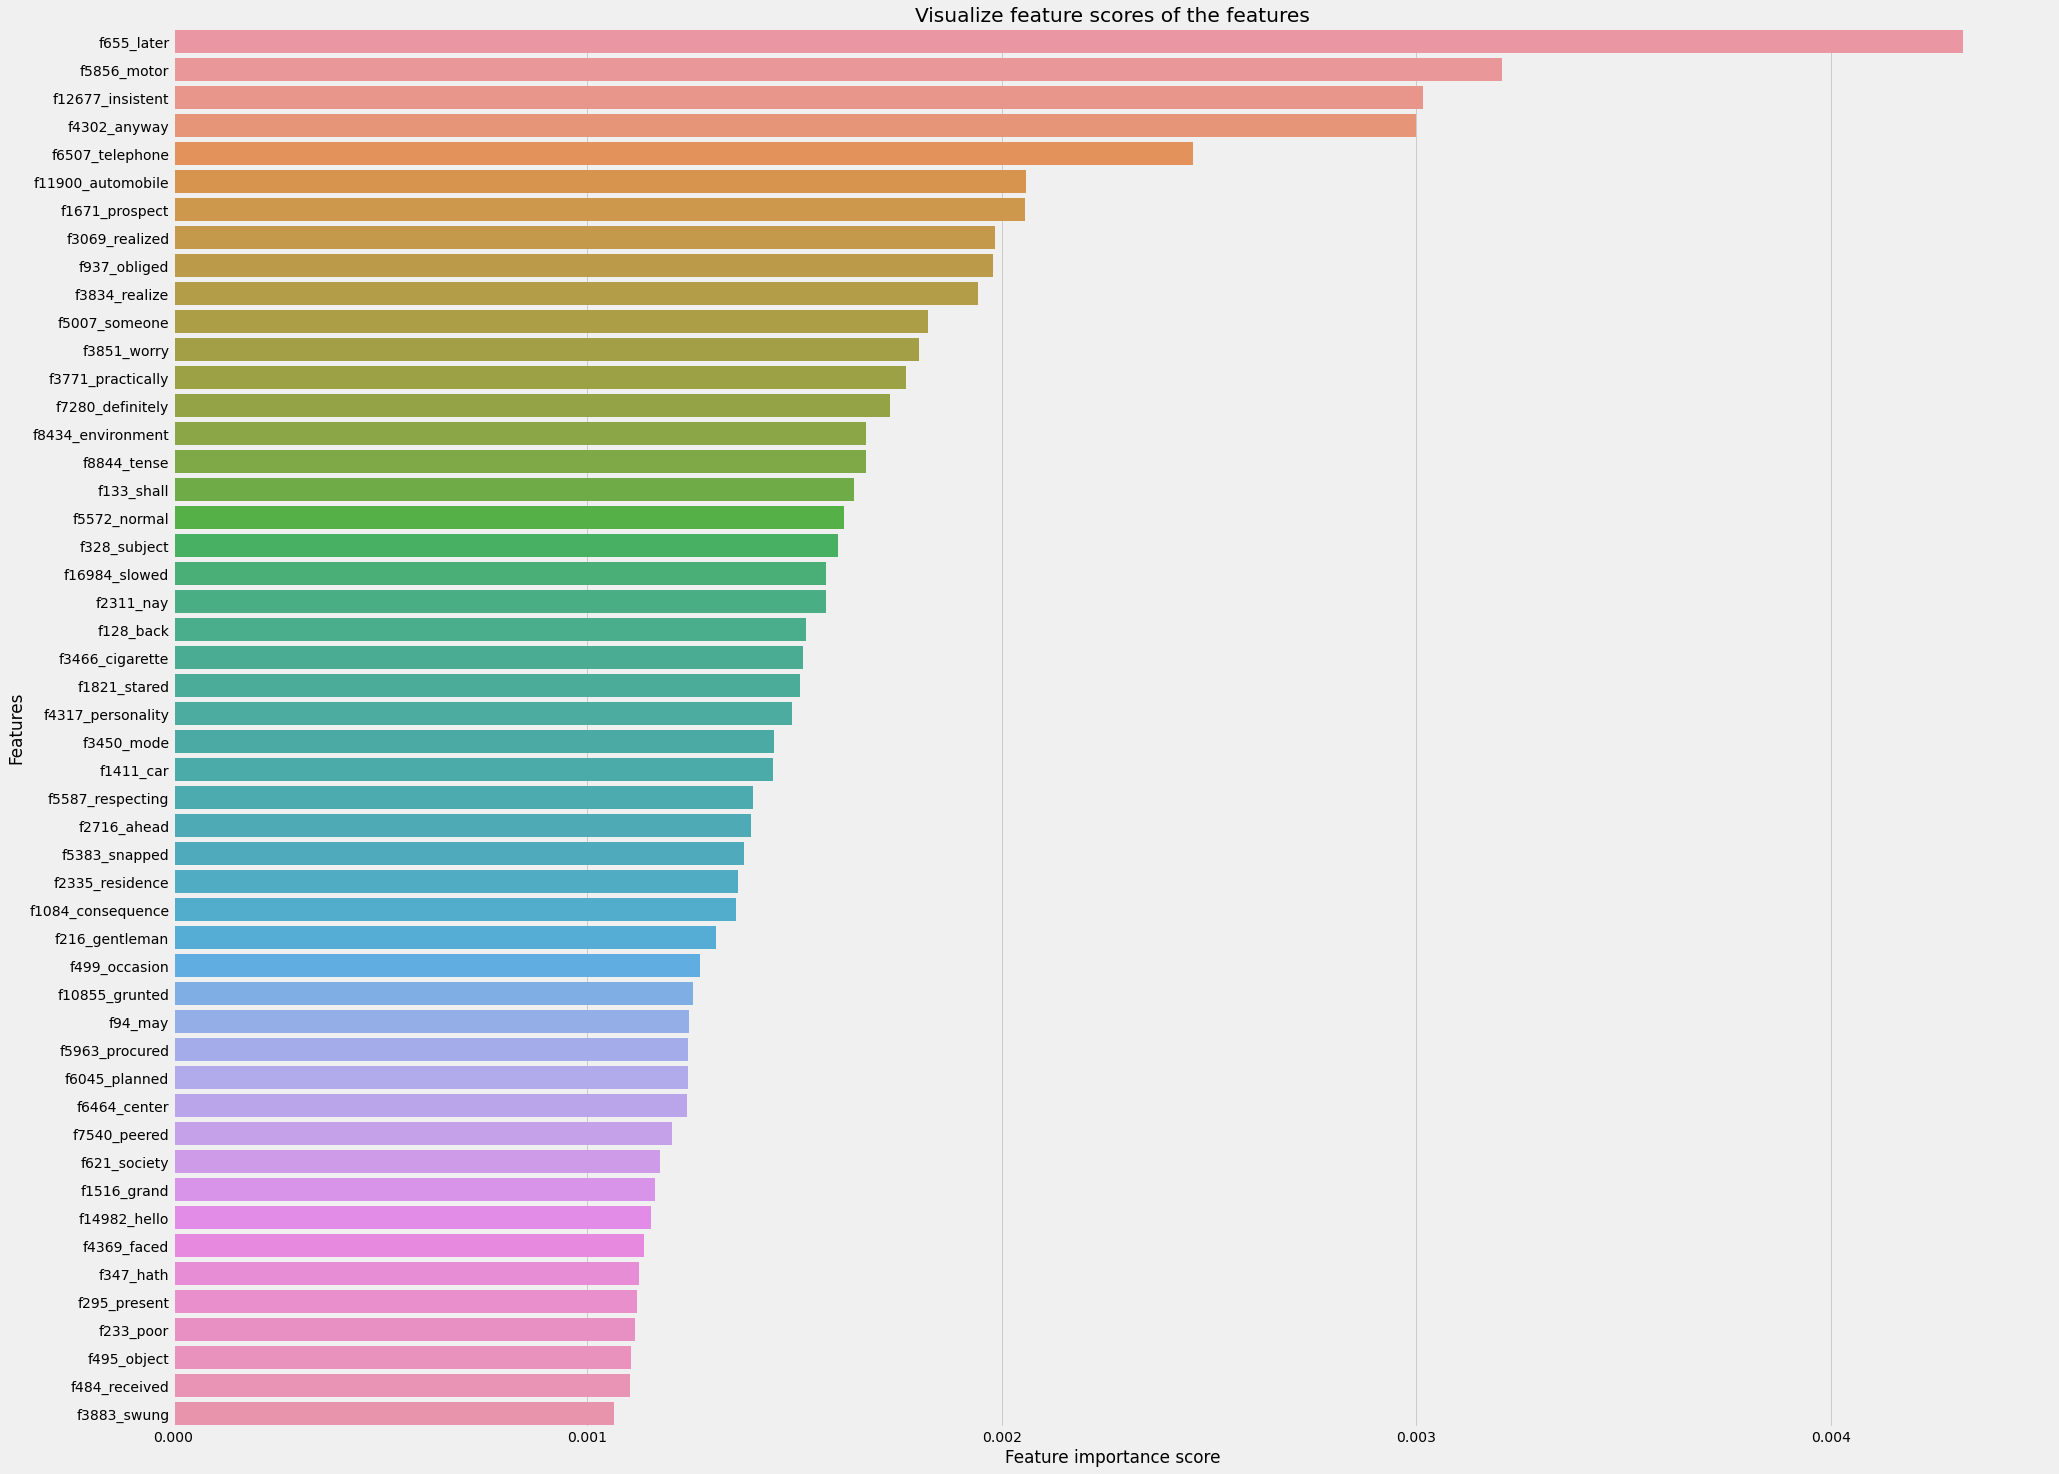
\includegraphics[width=0.5\textwidth]{figure1_featureVisualization.png}
  \caption{Feature Importance Random Forest}
  \end{figure}
=======
\subsection{Results}

Describe your experimental methodology (details about the data, preprocessing,
experimental methodology, and performance measures utilized).
>>>>>>> main

\begin{figure}[h]
  \centering
  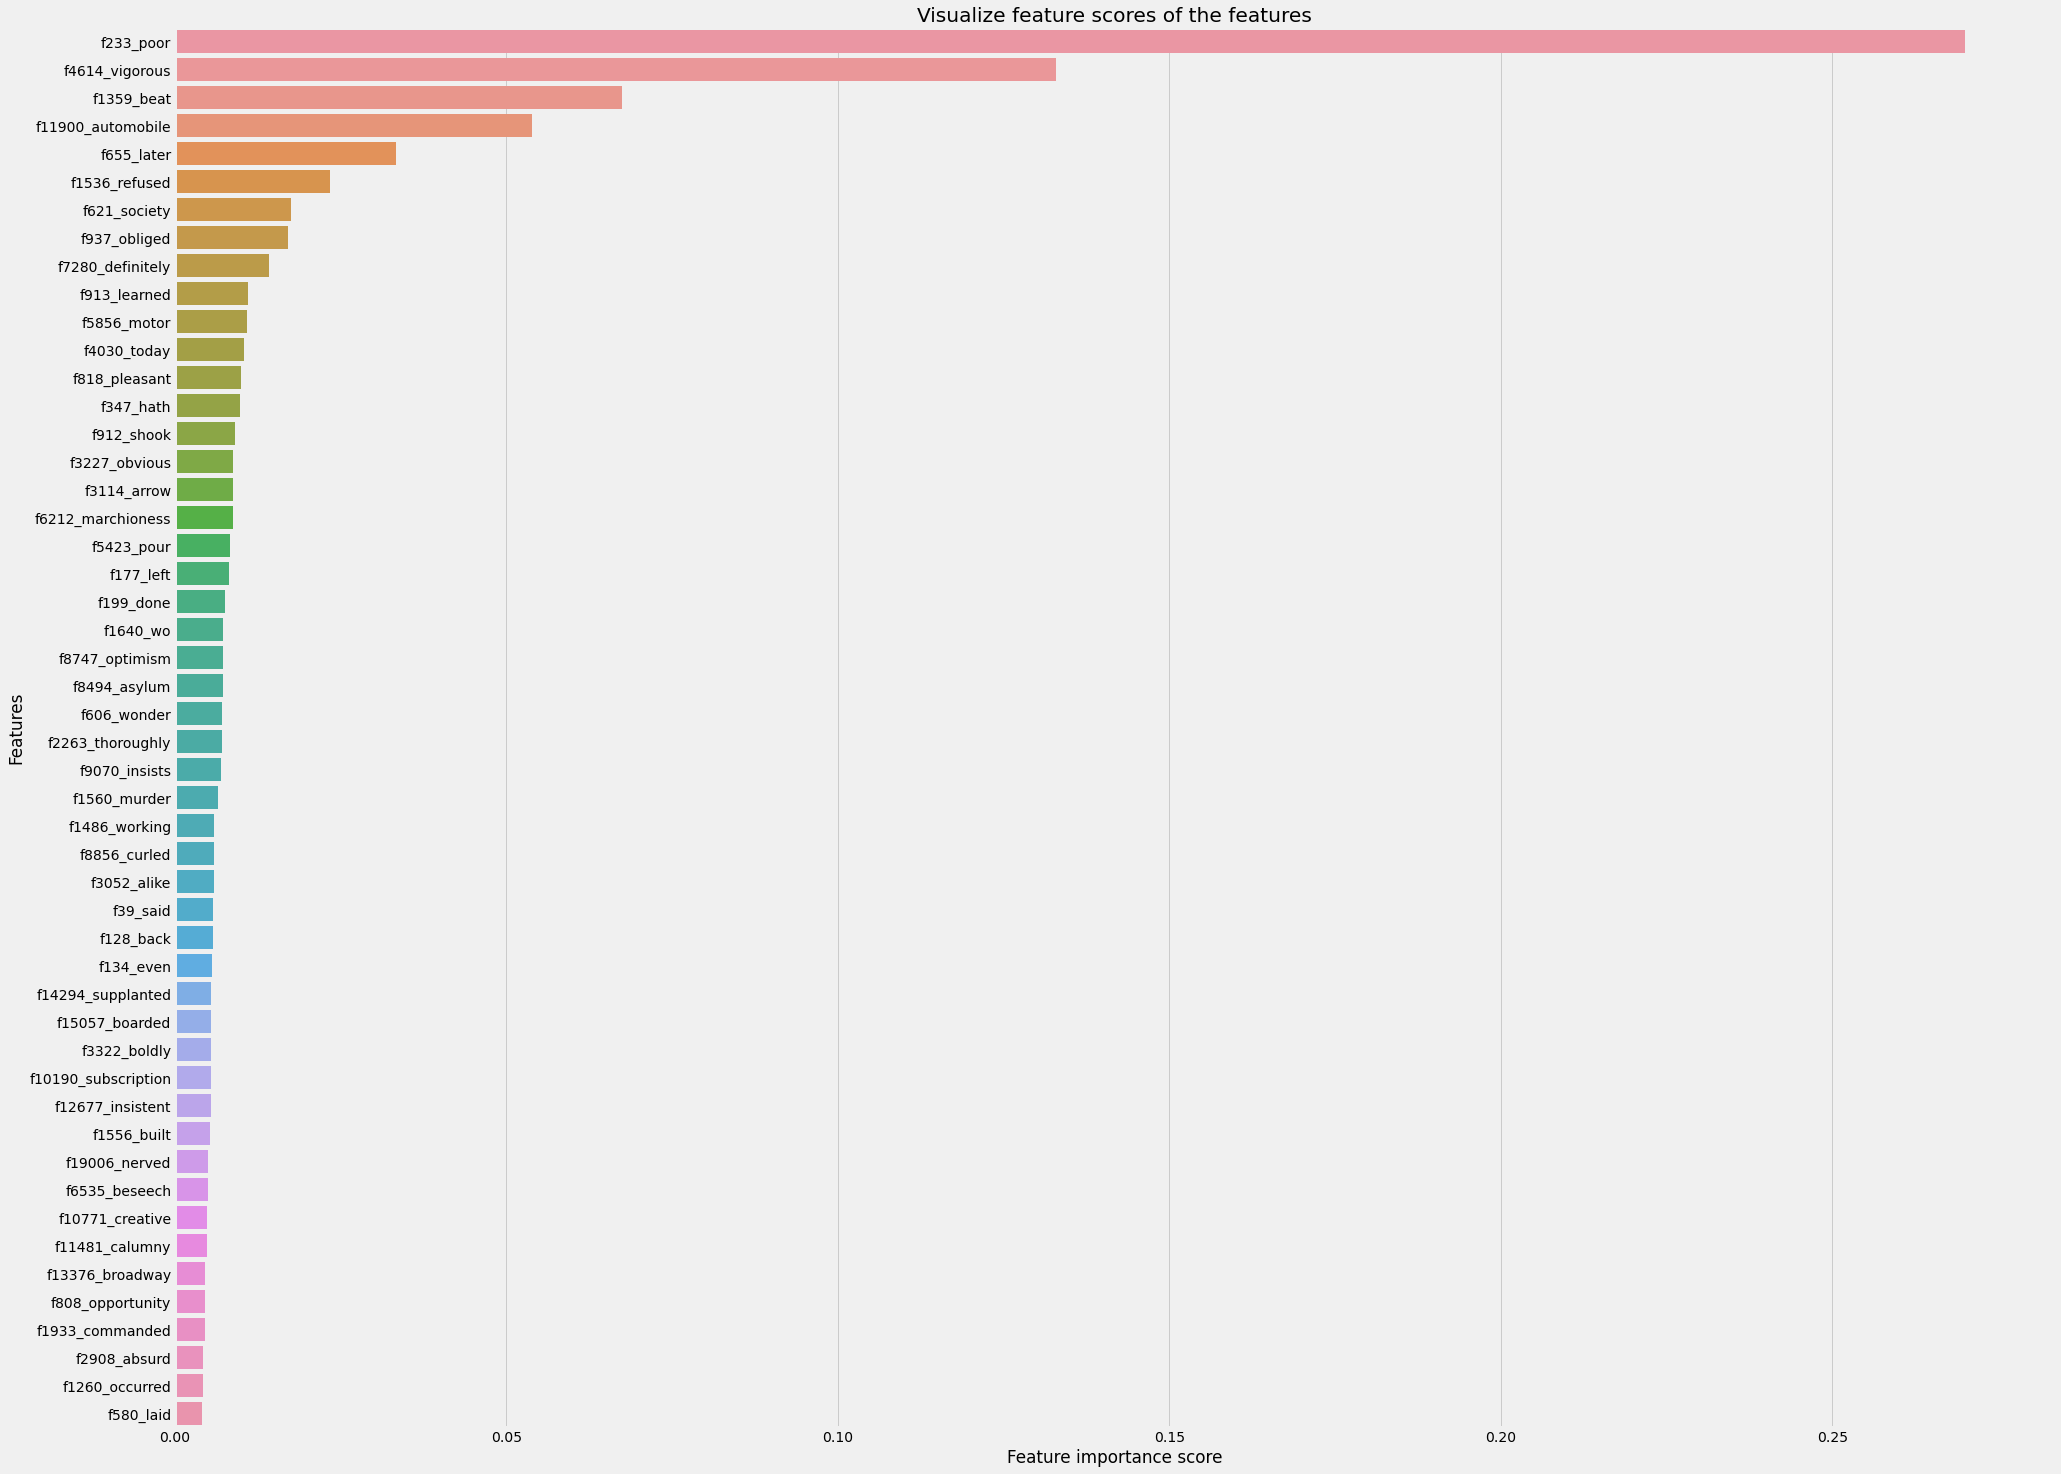
\includegraphics[width=0.5\textwidth]{feature_adaboost.png}
  \caption{Feature Importance AdaBoost}
  \end{figure}

The most notable difference between these two graphs is that the Random Forest classifier has a more even
distribution of MDI across the features while the AdaBoost classifier has a sharper decrease in MDI across
the features. Interestingly, seemingly innocuous words (e.g. poor and later) have the highest MDI values, In
addition to more archaic words (e.g. hath and alas) having significant MDI values. This could imply that the
decision trees initially split on commonly found words, and deeper into the trees do they diverge into more
obviously time specific language.

\section{Social Implications}

Our classification system has the potential to greatly impact 
the digital humanities community. 
Once unsolved problems could now, with some degree of reliability, be solved. Furthermore, as our system 
is not proprietary, those most interested in the subject may freely and openly
use and improve it. 
Therefore, it provides a resource to the 
digital humanities community that allows the individual to make discoveries, 
not just, say, a research group or well-funded corporation, providing 
an opportunity for those with deep interest in the subject to contribute 
when they may not have been able to before. 

That being said, a research group or corporation itself 
is made up of some number of individuals passionate about the material, and 
if this classification system is significantly better than their 
performance, this could lead to lower funding for these individuals.  


\section{Challenges}

We faced a number of challenges in designing and implementing our classification system. 
They can be broken down into the following categories:

\subsection{Design and Data Collection}

While our first challenge of finding a sufficient quantity of suitable data was very 
  easily solved, even the solution proved to have some difficulty. Due of the nature
  of the Project Gutenberg archive's structuring of meta-data associated with texts, 
  it was not possible for us to be able to find dates of original publish for each of
  the works that we encountered. As a solution, we resorted to manual
  labeling of data, which was high cost in terms of time-investment.

\subsection{Implementation}

Implementing the models also came with challenge. The first and most substantial 
was creating some standardized feature vector that allowed us to compare texts to each other. 
Without this, we would not be able to compare documents at all, as the same 
bucket in the feature vector for one document could stand for another feature in 
another document. After deliberation on how to best solve this problem, we 
developed the aforementioned standardized vector from a compilation of texts. 


\subsection{Testing and Validation}

In the case of training a model to do classification of texts based on something as abstracted 
  to the natural development of language as time period is, you end up with a problem where you are
  unable to accurately predict texts that should otherwise be classifiable because of the boundaries
  between two target labels being too close to a particular text's date of writing. An example would
  be that of a two texts, one written in 1899, and one written in 1900. Because of the cut-off boundary
  arbitrarily being between centuries, two texts which likely have more in common with each other than
  other texts of the same class as them end up being classified as two very different things. Coming up
  with solutions on how to mitigate this boundary error could help improve with accuracy over predictions.


\section{Conclusions}

Despite the high class imbalance of our dataset, thee relatively simply models have shown promising
results in text classification by time period. The Naive Bayes and Random forest models do well at 
distinguishing between texts <1899 and >1900, but are largely unable to classify texts outside of 
those time periods. The AdaBoost classifier seems to be able to classify texts outside of this time
range, and it is likely that with a larger and better balanced dataset, and higher complexity (e.g more estimators)
that its performance may increase. 

\subsection{Class Imbalance Issues}
Our original idea was to have several labels for a range of time periods, in order 
to better perfect our identification methods. However, we have a very bad case of 
sample balancing. This sample balancing is not something that could have been fixed 
by undersampling (this would cut down an extreme amount over the data that we have 
available), or oversampling (this would lead to extreme overfitting over the data 
that we do have available since we do not have a sufficient number of examples for 
these less sampled periods). Accordingly, we have cut down on the range of dates that 
we are processing. Instead, we are opting to do analysis per half-century between 
1800s and 1950s.

\section{Future Directions}

We believe that there is lots of room for improvement, but we have still accomplished 
good work in the way of our initial goal. There still exists issues, related to the project
that we have encountered that existed outside of the scope of what our plan developed into.
However, if we were to continue development outside of our four weeks, this is what we would 
consider:

\subsection{Feature Embedding}
Since we have such a high number of features, having some sort of feature embedding/feature
encoder feature reduction system would be very good for actually reducing the amount of 
data that we need to process. Because of the most common words appearing within a certain 
number of texts, there are many books which will simply exclude.

\subsection{Sample Rebalancing}
As mentioned in the conclusions section, we still have quite a few issues related to class 
balance. Perhaps we might be able to find higher accuracy over some of the more difficult to 
estimate time periods by sampling more evenly in terms of our data.

\subsection{Deep Learning}
With a larger and better balanced dataset, it may be possible o apply deep learning techniques
to model the time differences in texts. Deep learning models are well equipped to capture
spatio-temporal patterns in data, which may allow them to perform better at this type of
classification

\subsection{Feature Semantic Analysis}
The feature importance of the Random Forest and AdaBoost classifiers are measured by their Gini Index.
For a feature space of high cardinality, this may not be the best representation of feature importance.
Using different measures of feature importance, performing semantic analysis on important features may 
yield interesting results on what words or sets of words are most relevant at classifying texts
(e.g. the set of words relating to modern technology, or a set of old timey customary words)


\section*{Acknowledgments}

We would like to acknowledge our gratitude to the extensive and helpful oversight, advice, and support of Prof. Ben Mitchell
to this project, as well as the Swarthmore Computer Science Department for granting us 
access to department resources for this project. 



% In the unusual situation where you want a paper to appear in the
% references without citing it in the main text, use \nocite
\nocite{langley00}

\bibliography{references}
\bibliographystyle{icml2014}

\end{document}


% This document was modified from the file originally made available by
% Pat Langley and Andrea Danyluk for ICML-2K. This version was
% created by Lise Getoor and Tobias Scheffer, it was slightly modified
% from the 2010 version by Thorsten Joachims & Johannes Fuernkranz,
% slightly modified from the 2009 version by Kiri Wagstaff and
% Sam Roweis's 2008 version, which is slightly modified from
% Prasad Tadepalli's 2007 version which is a lightly
% changed version of the previous year's version by Andrew Moore,
% which was in turn edited from those of Kristian Kersting and
% Codrina Lauth. Alex Smola contributed to the algorithmic style files.
